\documentclass[
c,
11pt,
aspectratio=169, % 169 1610 149 32 43 54
final,
]{beamer}
\def\usebeamer{1}
\usepackage[T1]{fontenc}
\usepackage[utf8]{inputenc}
\usepackage[english,ngerman,shorthands=off]{babel}
\usepackage[autostyle]{csquotes}
\MakeOuterQuote{"}

\usepackage{amsmath}
% interesting options:
%   leqno Place equation numbers on the left.
%   reqno Place equation numbers on the right.
%   fleqn Position equations at a fixed indent from the left margin rather than centered in the text column
\usepackage{amsfonts, amsthm, amssymb}
\usepackage{xcolor}
\usepackage{fixmath} % fixes some Greek letters and provides \mathbold
\usepackage{mathtools}
\usepackage{lmodern}
%\usepackage{charter} % use charter font
\usepackage{ebgaramond}
\usepackage[tracking=true, % Fonts: hyphenatable letterspacing
expansion=true,            % Fonts: better grey value
protrusion=true,           % Fonts: margin kerning
babel]{microtype}
\usepackage{tikz,setspace}
\usetikzlibrary{calc,decorations.shapes}
\usepackage{pdfpages}
\usepackage{ifdraft} % provides \ifdraft
\usepackage{xifthen}
\usepackage{etoolbox}
\usepackage{longtable}
\usepackage{changepage}
\usepackage{emptypage} % clears headers/footers on empty pages
%\usepackage{pgfplots}\pgfplotsset{compat=1.13}
\usepackage{xfrac} % provides \sfrac for a/b
\usepackage{fix-cm} % fixes some font size issues
\usepackage[shortcuts]{extdash} % provides \-/ for breaking and \=/ for non-breaking hyphens
\usepackage{relsize}
\usepackage[rightcaption]{sidecap}
\usepackage{supertabular}
% \usepackage{natbib} % provides \citet, \citep

%\usepackage[osf,sc]{mathpazo}
%\usepackage{pdfcomment}
%\usepackage{flafter} % place floats at or after their appearance in code
\usepackage{booktabs} % better rules in tables
\usepackage{textcase} % provides \MakeTextUppercase
%\usepackage{silence} % provides \WarningFilter{PACKAGE}{WARNINGMESSAGE}
\usepackage[list=no]{caption}
\usepackage{graphicx}
\usepackage[position=top]{subfig}
\usepackage{adjustbox}
\usepackage{enumerate} % roman numbering in enumerations
\usepackage{colortbl} % color in tables
\usepackage{multirow}
%\usepackage{siunitx} % helps with SI units and number formats
\usepackage[section]{placeins} % provides \FloatBarrier to stop floats from passing certain barriers
%\usepackage{indentfirst} %	indent also the first paragraph of any chapter/section
\usepackage{url}
\usepackage{rotating}
\usepackage{subfiles}
\usepackage{anyfontsize}
\usepackage{hyphenat} % provides \nohyphens
\usepackage{fnpct} % nicer footnote typesetting
\usepackage{marginnote} % provides \marginnote
\usepackage{layout} % use with \layout to show current layout
% always include subfiles using \subfile
% these should look like
%   \documentclass[<mainfile>]{subfiles}
%   \begin{document}
%      ...
%   \end{document}
\usepackage[normalem]{ulem} % for underlining
\usepackage{gensymb}
\usepackage{xspace}
\usepackage{chngcntr} % provides \counterwithout
%\usepackage[backgroundcolor=white,bordercolor=none,textsize=small]{todonotes}

%\usepackage[mathlines]{lineno} % pagewise,modulo % enable numbering of text and display math
%\linenumbers

\frenchspacing % disabled additional space after periods
\clubpenalty = 10000 % disable single lines at the start of a paragraph (Schusterjungen)
\makeatletter
\@clubpenalty = 10000 % LaTeX uses `\@clubpenalty to restore the value of `\clubpenalty`
\makeatother
\widowpenalty 10000  % disable single lines at the end of a paragraph (Hurenkinder)
\displaywidowpenalty = 10000 % do not leave formulas alone
\raggedbottom % do not spread paragraphs
\numberwithin{equation}{section} % group equation numbering by section
%\numberwithin{figure}{chapter} % group figure numbering by section
%\usepackage[defaultlines=4,all]{nowidow}

% should be loaded last:
%\usepackage{varioref} % provides \vref as a "clever" reference for sections (e.g. on opposite page)
\usepackage{hyperref} % references as hyperlinks and provides \autoref to add "section", "figure", ... to \ref
% use \texorpdfstring{$E=mc^2$}{E=mc2} when necessary
\usepackage[nameinlink,noabbrev]{cleveref} % provides \cref{..,..} to add "section", "figure", ... to \ref and \crefrange{...}{...}, \cpageref, \cpagerefrange, \Cref, \labelref
%\usepackage{showkeys} % shows label and ref information for review (all 5 lines needed)
%\makeatletter
%  \SK@def\Cref#1{\SK@\SK@@ref{#1}\SK@Cref{#1}}%
%  \SK@def\cref#1{\SK@\SK@@ref{#1}\SK@cref{#1}}%
%\makeatother
% make sure to use the "right" commands:
%\let\ref\undefined
%\let\eqref\undefined
%\let\pageref\undefined

\hypersetup{pdfauthor={Christian Otto}}
\hypersetup{colorlinks=true}
\hypersetup{linkcolor=tableaured!50!black}
\hypersetup{urlcolor=tableaublue!50!black}
\hypersetup{citecolor=tableaublue!50!black}
\hypersetup{linktoc=all}

\definecolor{tableaublack}{HTML}{181818}
\definecolor{tableaublue}{HTML}{1F77B4}
\definecolor{tableauorange}{HTML}{FF7F0E}
\definecolor{tableaugreen}{HTML}{2CA02C}
\definecolor{tableaured}{HTML}{D62728}
\definecolor{tableaupurple}{HTML}{9467BD}
\definecolor{tableaubrown}{HTML}{8C564B}
\definecolor{tableaumagenta}{HTML}{E377C2}
\definecolor{tableaugray}{HTML}{7F7F7F}
\definecolor{tableaugrey}{HTML}{7F7F7F}
\definecolor{tableaulime}{HTML}{BCBD22}
\definecolor{tableaucyan}{HTML}{17BECF}
\definecolor{tableaulightblue}{HTML}{AEC7E8}
\definecolor{tableaulightorange}{HTML}{FFBB78}
\definecolor{tableaulightgreen}{HTML}{98DF8A}
\definecolor{tableaulightred}{HTML}{FF9896}
\definecolor{tableaulightpurple}{HTML}{C5B0D5}
\definecolor{tableaulightbrown}{HTML}{C49C94}
\definecolor{tableaulightmagenta}{HTML}{F7B6D2}
\definecolor{tableaulightgray}{HTML}{C7C7C7}
\definecolor{tableaulightgrey}{HTML}{C7C7C7}
\definecolor{tableaulightlime}{HTML}{DBDB8D}
\definecolor{tableaulightcyan}{HTML}{9EDAE5}

% files including header should also include:
% \usepackage[T1]{fontenc}
\usepackage[utf8]{inputenc}
\usepackage[english,ngerman,shorthands=off]{babel}
\usepackage[autostyle]{csquotes}
\MakeOuterQuote{"}

\usepackage{amsmath}
% interesting options:
%   leqno Place equation numbers on the left.
%   reqno Place equation numbers on the right.
%   fleqn Position equations at a fixed indent from the left margin rather than centered in the text column
\usepackage{amsfonts, amsthm, amssymb}
\usepackage{xcolor}
\usepackage{fixmath} % fixes some Greek letters and provides \mathbold
\usepackage{mathtools}
\usepackage{lmodern}
%\usepackage{charter} % use charter font
\usepackage{ebgaramond}
\usepackage[tracking=true, % Fonts: hyphenatable letterspacing
expansion=true,            % Fonts: better grey value
protrusion=true,           % Fonts: margin kerning
babel]{microtype}
\usepackage{tikz,setspace}
\usetikzlibrary{calc,decorations.shapes}
\usepackage{pdfpages}
\usepackage{ifdraft} % provides \ifdraft
\usepackage{xifthen}
\usepackage{etoolbox}
\usepackage{longtable}
\usepackage{changepage}
\usepackage{emptypage} % clears headers/footers on empty pages
%\usepackage{pgfplots}\pgfplotsset{compat=1.13}
\usepackage{xfrac} % provides \sfrac for a/b
\usepackage{fix-cm} % fixes some font size issues
\usepackage[shortcuts]{extdash} % provides \-/ for breaking and \=/ for non-breaking hyphens
\usepackage{relsize}
\usepackage[rightcaption]{sidecap}
\usepackage{supertabular}
% \usepackage{natbib} % provides \citet, \citep

%\usepackage[osf,sc]{mathpazo}
%\usepackage{pdfcomment}
%\usepackage{flafter} % place floats at or after their appearance in code
\usepackage{booktabs} % better rules in tables
\usepackage{textcase} % provides \MakeTextUppercase
%\usepackage{silence} % provides \WarningFilter{PACKAGE}{WARNINGMESSAGE}
\usepackage[list=no]{caption}
\usepackage{graphicx}
\usepackage[position=top]{subfig}
\usepackage{adjustbox}
\usepackage{enumerate} % roman numbering in enumerations
\usepackage{colortbl} % color in tables
\usepackage{multirow}
%\usepackage{siunitx} % helps with SI units and number formats
\usepackage[section]{placeins} % provides \FloatBarrier to stop floats from passing certain barriers
%\usepackage{indentfirst} %	indent also the first paragraph of any chapter/section
\usepackage{url}
\usepackage{rotating}
\usepackage{subfiles}
\usepackage{anyfontsize}
\usepackage{hyphenat} % provides \nohyphens
\usepackage{fnpct} % nicer footnote typesetting
\usepackage{marginnote} % provides \marginnote
\usepackage{layout} % use with \layout to show current layout
% always include subfiles using \subfile
% these should look like
%   \documentclass[<mainfile>]{subfiles}
%   \begin{document}
%      ...
%   \end{document}
\usepackage[normalem]{ulem} % for underlining
\usepackage{gensymb}
\usepackage{xspace}
\usepackage{chngcntr} % provides \counterwithout
%\usepackage[backgroundcolor=white,bordercolor=none,textsize=small]{todonotes}

%\usepackage[mathlines]{lineno} % pagewise,modulo % enable numbering of text and display math
%\linenumbers

\frenchspacing % disabled additional space after periods
\clubpenalty = 10000 % disable single lines at the start of a paragraph (Schusterjungen)
\makeatletter
\@clubpenalty = 10000 % LaTeX uses `\@clubpenalty to restore the value of `\clubpenalty`
\makeatother
\widowpenalty 10000  % disable single lines at the end of a paragraph (Hurenkinder)
\displaywidowpenalty = 10000 % do not leave formulas alone
\raggedbottom % do not spread paragraphs
\numberwithin{equation}{section} % group equation numbering by section
%\numberwithin{figure}{chapter} % group figure numbering by section
%\usepackage[defaultlines=4,all]{nowidow}

% should be loaded last:
%\usepackage{varioref} % provides \vref as a "clever" reference for sections (e.g. on opposite page)
\usepackage{hyperref} % references as hyperlinks and provides \autoref to add "section", "figure", ... to \ref
% use \texorpdfstring{$E=mc^2$}{E=mc2} when necessary
\usepackage[nameinlink,noabbrev]{cleveref} % provides \cref{..,..} to add "section", "figure", ... to \ref and \crefrange{...}{...}, \cpageref, \cpagerefrange, \Cref, \labelref
%\usepackage{showkeys} % shows label and ref information for review (all 5 lines needed)
%\makeatletter
%  \SK@def\Cref#1{\SK@\SK@@ref{#1}\SK@Cref{#1}}%
%  \SK@def\cref#1{\SK@\SK@@ref{#1}\SK@cref{#1}}%
%\makeatother
% make sure to use the "right" commands:
%\let\ref\undefined
%\let\eqref\undefined
%\let\pageref\undefined

\hypersetup{pdfauthor={Christian Otto}}
\hypersetup{colorlinks=true}
\hypersetup{linkcolor=tableaured!50!black}
\hypersetup{urlcolor=tableaublue!50!black}
\hypersetup{citecolor=tableaublue!50!black}
\hypersetup{linktoc=all}

\definecolor{tableaublack}{HTML}{181818}
\definecolor{tableaublue}{HTML}{1F77B4}
\definecolor{tableauorange}{HTML}{FF7F0E}
\definecolor{tableaugreen}{HTML}{2CA02C}
\definecolor{tableaured}{HTML}{D62728}
\definecolor{tableaupurple}{HTML}{9467BD}
\definecolor{tableaubrown}{HTML}{8C564B}
\definecolor{tableaumagenta}{HTML}{E377C2}
\definecolor{tableaugray}{HTML}{7F7F7F}
\definecolor{tableaugrey}{HTML}{7F7F7F}
\definecolor{tableaulime}{HTML}{BCBD22}
\definecolor{tableaucyan}{HTML}{17BECF}
\definecolor{tableaulightblue}{HTML}{AEC7E8}
\definecolor{tableaulightorange}{HTML}{FFBB78}
\definecolor{tableaulightgreen}{HTML}{98DF8A}
\definecolor{tableaulightred}{HTML}{FF9896}
\definecolor{tableaulightpurple}{HTML}{C5B0D5}
\definecolor{tableaulightbrown}{HTML}{C49C94}
\definecolor{tableaulightmagenta}{HTML}{F7B6D2}
\definecolor{tableaulightgray}{HTML}{C7C7C7}
\definecolor{tableaulightgrey}{HTML}{C7C7C7}
\definecolor{tableaulightlime}{HTML}{DBDB8D}
\definecolor{tableaulightcyan}{HTML}{9EDAE5}

% files including header should also include:
% \usepackage[T1]{fontenc}
\usepackage[utf8]{inputenc}
\usepackage[english,ngerman,shorthands=off]{babel}
\usepackage[autostyle]{csquotes}
\MakeOuterQuote{"}

\usepackage{amsmath}
% interesting options:
%   leqno Place equation numbers on the left.
%   reqno Place equation numbers on the right.
%   fleqn Position equations at a fixed indent from the left margin rather than centered in the text column
\usepackage{amsfonts, amsthm, amssymb}
\usepackage{xcolor}
\usepackage{fixmath} % fixes some Greek letters and provides \mathbold
\usepackage{mathtools}
\usepackage{lmodern}
%\usepackage{charter} % use charter font
\usepackage{ebgaramond}
\usepackage[tracking=true, % Fonts: hyphenatable letterspacing
expansion=true,            % Fonts: better grey value
protrusion=true,           % Fonts: margin kerning
babel]{microtype}
\usepackage{tikz,setspace}
\usetikzlibrary{calc,decorations.shapes}
\usepackage{pdfpages}
\usepackage{ifdraft} % provides \ifdraft
\usepackage{xifthen}
\usepackage{etoolbox}
\usepackage{longtable}
\usepackage{changepage}
\usepackage{emptypage} % clears headers/footers on empty pages
%\usepackage{pgfplots}\pgfplotsset{compat=1.13}
\usepackage{xfrac} % provides \sfrac for a/b
\usepackage{fix-cm} % fixes some font size issues
\usepackage[shortcuts]{extdash} % provides \-/ for breaking and \=/ for non-breaking hyphens
\usepackage{relsize}
\usepackage[rightcaption]{sidecap}
\usepackage{supertabular}
% \usepackage{natbib} % provides \citet, \citep

%\usepackage[osf,sc]{mathpazo}
%\usepackage{pdfcomment}
%\usepackage{flafter} % place floats at or after their appearance in code
\usepackage{booktabs} % better rules in tables
\usepackage{textcase} % provides \MakeTextUppercase
%\usepackage{silence} % provides \WarningFilter{PACKAGE}{WARNINGMESSAGE}
\usepackage[list=no]{caption}
\usepackage{graphicx}
\usepackage[position=top]{subfig}
\usepackage{adjustbox}
\usepackage{enumerate} % roman numbering in enumerations
\usepackage{colortbl} % color in tables
\usepackage{multirow}
%\usepackage{siunitx} % helps with SI units and number formats
\usepackage[section]{placeins} % provides \FloatBarrier to stop floats from passing certain barriers
%\usepackage{indentfirst} %	indent also the first paragraph of any chapter/section
\usepackage{url}
\usepackage{rotating}
\usepackage{subfiles}
\usepackage{anyfontsize}
\usepackage{hyphenat} % provides \nohyphens
\usepackage{fnpct} % nicer footnote typesetting
\usepackage{marginnote} % provides \marginnote
\usepackage{layout} % use with \layout to show current layout
% always include subfiles using \subfile
% these should look like
%   \documentclass[<mainfile>]{subfiles}
%   \begin{document}
%      ...
%   \end{document}
\usepackage[normalem]{ulem} % for underlining
\usepackage{gensymb}
\usepackage{xspace}
\usepackage{chngcntr} % provides \counterwithout
%\usepackage[backgroundcolor=white,bordercolor=none,textsize=small]{todonotes}

%\usepackage[mathlines]{lineno} % pagewise,modulo % enable numbering of text and display math
%\linenumbers

\frenchspacing % disabled additional space after periods
\clubpenalty = 10000 % disable single lines at the start of a paragraph (Schusterjungen)
\makeatletter
\@clubpenalty = 10000 % LaTeX uses `\@clubpenalty to restore the value of `\clubpenalty`
\makeatother
\widowpenalty 10000  % disable single lines at the end of a paragraph (Hurenkinder)
\displaywidowpenalty = 10000 % do not leave formulas alone
\raggedbottom % do not spread paragraphs
\numberwithin{equation}{section} % group equation numbering by section
%\numberwithin{figure}{chapter} % group figure numbering by section
%\usepackage[defaultlines=4,all]{nowidow}

% should be loaded last:
%\usepackage{varioref} % provides \vref as a "clever" reference for sections (e.g. on opposite page)
\usepackage{hyperref} % references as hyperlinks and provides \autoref to add "section", "figure", ... to \ref
% use \texorpdfstring{$E=mc^2$}{E=mc2} when necessary
\usepackage[nameinlink,noabbrev]{cleveref} % provides \cref{..,..} to add "section", "figure", ... to \ref and \crefrange{...}{...}, \cpageref, \cpagerefrange, \Cref, \labelref
%\usepackage{showkeys} % shows label and ref information for review (all 5 lines needed)
%\makeatletter
%  \SK@def\Cref#1{\SK@\SK@@ref{#1}\SK@Cref{#1}}%
%  \SK@def\cref#1{\SK@\SK@@ref{#1}\SK@cref{#1}}%
%\makeatother
% make sure to use the "right" commands:
%\let\ref\undefined
%\let\eqref\undefined
%\let\pageref\undefined

\hypersetup{pdfauthor={Christian Otto}}
\hypersetup{colorlinks=true}
\hypersetup{linkcolor=tableaured!50!black}
\hypersetup{urlcolor=tableaublue!50!black}
\hypersetup{citecolor=tableaublue!50!black}
\hypersetup{linktoc=all}

\definecolor{tableaublack}{HTML}{181818}
\definecolor{tableaublue}{HTML}{1F77B4}
\definecolor{tableauorange}{HTML}{FF7F0E}
\definecolor{tableaugreen}{HTML}{2CA02C}
\definecolor{tableaured}{HTML}{D62728}
\definecolor{tableaupurple}{HTML}{9467BD}
\definecolor{tableaubrown}{HTML}{8C564B}
\definecolor{tableaumagenta}{HTML}{E377C2}
\definecolor{tableaugray}{HTML}{7F7F7F}
\definecolor{tableaugrey}{HTML}{7F7F7F}
\definecolor{tableaulime}{HTML}{BCBD22}
\definecolor{tableaucyan}{HTML}{17BECF}
\definecolor{tableaulightblue}{HTML}{AEC7E8}
\definecolor{tableaulightorange}{HTML}{FFBB78}
\definecolor{tableaulightgreen}{HTML}{98DF8A}
\definecolor{tableaulightred}{HTML}{FF9896}
\definecolor{tableaulightpurple}{HTML}{C5B0D5}
\definecolor{tableaulightbrown}{HTML}{C49C94}
\definecolor{tableaulightmagenta}{HTML}{F7B6D2}
\definecolor{tableaulightgray}{HTML}{C7C7C7}
\definecolor{tableaulightgrey}{HTML}{C7C7C7}
\definecolor{tableaulightlime}{HTML}{DBDB8D}
\definecolor{tableaulightcyan}{HTML}{9EDAE5}

% files including header should also include:
% \input{header}
% \title{}
% \author{}
% \hypersetup{pdftitle={}}
% \hypersetup{pdfsubject={}}
% \hypersetup{pdfkeywords={}{}{}}
% \graphicspath{{./figures/}}
% ...
% \bibliographystyle{plainnat}

% \ifx\whatsoever\empty\relax\else\relax\fi
\hyphenation{dis-equi-lib-ri-um dis-ag-gre-gat-ed dis-ag-gre-gate dis-ag-gre-ga-tion adap-ta-tion mod-el ac-cli-mate}

\urlstyle{customurl}

%%% Local Variables:
%%% mode: latex
%%% TeX-master: "../thesis"
%%% TeX-command-default: "Make"
%%% End:

% \title{}
% \author{}
% \hypersetup{pdftitle={}}
% \hypersetup{pdfsubject={}}
% \hypersetup{pdfkeywords={}{}{}}
% \graphicspath{{./figures/}}
% ...
% \bibliographystyle{plainnat}

% \ifx\whatsoever\empty\relax\else\relax\fi
\hyphenation{dis-equi-lib-ri-um dis-ag-gre-gat-ed dis-ag-gre-gate dis-ag-gre-ga-tion adap-ta-tion mod-el ac-cli-mate}

\urlstyle{customurl}

%%% Local Variables:
%%% mode: latex
%%% TeX-master: "../thesis"
%%% TeX-command-default: "Make"
%%% End:

% \title{}
% \author{}
% \hypersetup{pdftitle={}}
% \hypersetup{pdfsubject={}}
% \hypersetup{pdfkeywords={}{}{}}
% \graphicspath{{./figures/}}
% ...
% \bibliographystyle{plainnat}

% \ifx\whatsoever\empty\relax\else\relax\fi
\hyphenation{dis-equi-lib-ri-um dis-ag-gre-gat-ed dis-ag-gre-gate dis-ag-gre-ga-tion adap-ta-tion mod-el ac-cli-mate}

\urlstyle{customurl}

%%% Local Variables:
%%% mode: latex
%%% TeX-master: "../thesis"
%%% TeX-command-default: "Make"
%%% End:

\linespread{1.2}
% \newboolean{consumer}
% \newboolean{onlyagent}
% \newboolean{showshock}

% \def\nobackupslides{true}

% \setbeameroption{show notes on second screen}
% \setbeameroption{show notes}
% \includeonlyframes{stateoftheart,contributions}\renewcommand{\note}[2][1]{}

\usepackage[framemethod=TikZ]{mdframed}
\usepackage[default]{lato}
\usepackage{multicol}
\usepackage[nomessages]{fp}
\usepackage{sfmath}
\usepackage{marvosym} % \MVRightarrow
\usepackage{pgfpages}
\usepackage[duration=8]{pdfpcnotes}
% \usepackage{pdfpc-commands}

\makeatletter

% switch default weight to light
\renewcommand{\mddefault}{m}
\renewcommand{\bfdefault}{m}

% Lengths:
\newlength{\borderheight}
\newlength{\cornerradius}
\newlength{\fullframewidth}
\newlength{\leftframemargin}
\newlength{\maxfigureheight}
\newlength{\outlinewidth}
\newlength{\rightframemargin}
\newlength{\zoomoverlaygap}
\newlength{\zoomoverlayheight}
\newlength{\zoomoverlayshift}
\newlength{\zoomoverlaywidth}
\setlength{\borderheight}{8mm}
\setlength{\cornerradius}{0.6mm}
\setlength{\fboxsep}{0mm}
\setlength{\fullframewidth}{\textwidth+\Gm@lmargin+\Gm@rmargin}
\setlength{\leftframemargin}{\Gm@lmargin}
\setlength{\maxfigureheight}{0.75\paperheight}
\setlength{\outlinewidth}{0.5mm}
\setlength{\rightframemargin}{\Gm@rmargin}
\setlength{\zoomoverlaygap}{5mm}
\setlength{\zoomoverlayheight}{\zoomoverlaywidth/3*2}
\setlength{\zoomoverlayshift}{-10mm}
\setlength{\zoomoverlaywidth}{50mm}

\setbeamercolor{background canvas}{bg = white}
\setbeamercolor{normal text}{fg = black}
\setbeamercolor{frametitle}{fg = tableaublue!80!black}
\setbeamercolor{title}{fg = black}
\setbeamercolor{section title}{fg = black}
\setbeamercolor{section in toc}{fg = black}
\setbeamercolor{section in toc shaded}{fg = black}
\setbeamercolor{enumerate item}{fg = tableaublue}
\setbeamercolor{enumerate subitem}{fg = tableaublue}
\setbeamercolor{enumerate subsubitem}{fg = tableaublue}
\setbeamercolor{itemize item}{fg = tableaublue}
\setbeamercolor{itemize subitem}{fg = tableauorange}
\setbeamercolor{itemize subsubitem}{fg = tableaugreen}
\setbeamercolor{caption name}{fg = tableaublue}
\setbeamercolor{block title}{fg = tableaublue}
\setbeamercolor{block title example}{fg = tableaugreen}

\setbeamerfont{frametitle}{size=\fontsize{13pt}{14pt},series=\bfseries}
\setbeamerfont{footline}{size=\fontsize{7pt}{7pt}}
\setbeamerfont{normal text}{size=\fontsize{11pt}{11pt}}
\setbeamerfont{enumerate item}{series=\bfseries}

\setbeamertemplate{items}[square]
\setbeamertemplate{itemize item}{\tikz{\clip (-.04,-.04) rectangle (.2,.2);\fill[color=tableaublue] rectangle(.18,.18);}}
\setbeamertemplate{itemize subitem}{\tikz{\clip (-.04,-.04) rectangle (.18,.18);\fill[color=tableauorange] rectangle(.16,.16);}}
\setbeamertemplate{itemize subsubitem}{\tikz{\clip (-.04,-.04) rectangle (.16,.16);\fill[color=tableaugreen] rectangle(.14,.14);}}
\setbeamertemplate{enumerate items}[default]
\setbeamertemplate{blocks}[rounded][shadow=false]
\setbeamertemplate{navigation symbols}{}
% \newenvironment{xplainframe}\frametitle{\bgroup\setbeamertemplate{background}{}\begin{frame}[plain]}{\end{frame}\egroup}
\setbeamertemplate{headline}{\includeedges}
\setbeamertemplate{sidebar canvas right}{}
\setbeamertemplate{frametitle}{\vspace*{6mm}\hspace{-1.5mm}\insertframetitle\vspace{2.5mm}}
\setbeamertemplate{footline}{\vbox to \borderheight {}}
\setbeamertemplate{note page}{
  \insertslideintonotes{0.4}\par
  {\large\insertframetitle}\par
  %\hrule\par
  \insertnote
}
\setbeamertemplate{title page}{
  \tikz[baseline,overlay]{
    \node[align=center] at ( $(current page.center)+(0mm,5mm)$ ) {%
      \fontsize{17pt}{21pt}\selectfont
      \textcolor{tableaublue}{\textbf{\inserttitle}}
    };
    % \node[align=center] at ( $(current page.center)+(0mm,-5mm)$) {%
    %   \fontsize{15pt}{16pt}\selectfont
    %   \textcolor{black}{\insertsubtitle}
    % };
    \node[align=center] at ( $(current page.center)+(0mm,-20mm)$ ) {%
      \begin{minipage}{10cm}
        \centering
        \fontsize{11pt}{15pt}\selectfont
        \textcolor{black}{\insertauthor}\\[1cm]
        \fontsize{11pt}{15pt}\selectfont
        \textcolor{tableaublue}{\insertdate}
      \end{minipage}
    };
  }
  \includeedges[0]
}
\setbeamertemplate{section page}{%
  \vskip1cm
  \begin{centering}
    \begin{beamercolorbox}[sep=12pt,center]{section title}
      \usebeamerfont{section title}\insertsection\par
    \end{beamercolorbox}
  \end{centering}
}

\usetikzlibrary{
  arrows,
  arrows.meta,
  shapes.geometric,
  positioning,
  fit,
  calc,
  decorations.shapes,
  decorations.pathreplacing
}

\hypersetup{pdfpagemode=UseNone} % don't show bookmarks on initial view
\tikzstyle{every picture}+=[remember picture]
\everymath{\displaystyle}

\DeclareDocumentCommand{\overlay}{ O{north west} O{north west} m m }{
  \tikz[baseline,overlay]\node[shift={(#3)},anchor=#2] at (current page.#1) {%]
    #4%
    \par\vspace{0mm}
  };
}

\DeclareDocumentEnvironment{overlay}{ O{north west} O{north west} m }{
  \tikz[baseline,overlay]\node[shift={(#3)},align=left,anchor=#2] at (current page.#1) \bgroup
}{
  \par\vspace{0mm}
  \egroup;
}

\newcommand{\drawmapcorrection}{
  \tikz[baseline,overlay]{
    \fill[fill=white] ($(current page.west)+(1mm,-7mm)$) rectangle ($(current page.west)+(22mm,13mm)$);
    \fill[fill=white] ($(current page.east)+(-31mm,-12mm)$) rectangle ($(current page.east)+(-28mm,-5mm)$);
    \fill[fill=white] ($(current page.center)+(7mm,-23mm)$) rectangle ($(current page.center)+(14mm,-17mm)$);
  }
}

\newcommand{\arrowitem}{\item[\raisebox{0.75pt}{\MVRightarrow}]}

\DeclareDocumentCommand{\culine}{ O{1pt} O{-0.75ex} m }{%
  \bgroup\markoverwith{\textcolor{#3}{\rule[#2]{2pt}{#1}}}\ULon%
}

\newcommand{\anchor}[1]{\tikz\node[coordinate] (#1) {};}
\DeclareDocumentCommand{\connect}{ O{->} O{} m m }{
  \tikz[baseline,overlay]\path[#1] (#3) edge[#2] (#4);
}

\DeclareDocumentCommand{\addfooter}{ m }{
  \begin{overlay}[south east][east]{-6mm,\borderheight/2-0.025}
    \textcolor{white}{
      \fontsize{7pt}{7pt}\selectfont
      #1
    }
  \end{overlay}
}

\DeclareDocumentEnvironment{messages}{ O{-3mm} }{
  %\begin{overlay}[south][south]{0mm,\borderheight-4.5mm}
  %\begin{minipage}{0.65\textwidth}
  \begin{itemize}
    \centering\vspace{#1}
    \setlength{\itemsep}{0.2em}
  }{
  \end{itemize}
  % \end{minipage}
  % \end{overlay}
}

\DeclareDocumentCommand{\formatsource}{ O{} m m m m }{
  % #1 (#2). \textbf{#3}, #4.
  \textbf{#2 (#3)}%
  \ifthenelse{\equal{#1}{nodot}}{}{.}
}

\newsavebox{\sourcesbox}
\DeclareDocumentEnvironment{sources}{}{
  \begin{overlay}[south east][south east]{-9mm,\borderheight-5.5mm}
    % \begin{lrbox}{\sourcesbox}
    \begin{minipage}{\textwidth}
      \fontsize{7.5pt}{10pt}\selectfont
      \begin{itemize}
        \setlength{\itemsep}{0.3em}
        \raggedleft
      }{
      \end{itemize}
      \mbox{}
    \end{minipage}
    % \end{lrbox}
    % \begin{overlay}[south east][south east]{-6mm,\borderheight-1.67mm}
    %   \usebox{\sourcesbox}
  \end{overlay}
  % \phantom{
  % \usebox{\sourcesbox}
  % }
}

\DeclareDocumentCommand{\includeedges}{ O{1} }{
  \tikz[baseline,overlay]{
    \ifthenelse{\equal{#1}{1}}{
      \draw[color=black,opacity=0.6] ($(current page.south west)+(22mm,\borderheight)$) -- ($(current page.south east)+(-11mm,\borderheight)$);
      \node[anchor=west,inner sep=0] at ($(current page.south west)+(3mm,\borderheight-1.02mm)$) {%
        
\includegraphics[width=17.5mm]{figures/logo_pik_small}
      };
      \node[anchor=west,inner sep=0] at ($(current page.south west)+(68mm,\borderheight/2)$) {%
        %\includegraphics[height=4mm]{figures/logo_rd4}
      };
      \node[anchor=west,opacity=0.6] at ( $(current page.south west)+(78mm,\borderheight/2)$) {%
          \insertdate
      };
      \node[anchor=east,opacity=0.6] at ( $(current page.south east)+(-11mm,\borderheight/2)$) {%
        % \insertpagenumber
        \insertframenumber
      };
    }{
      \node[anchor=north west,inner sep=0] at ($(current page.north west)+(4mm,-11.5mm)$) {%
        
\includegraphics[width=80mm]{figures/logo_pik}
      };
      % \draw[color=black,opacity=0.6] ($(current page.south west)+(3mm,15mm)$) -- ($(current page.south east)+(-3mm,15mm)$);
      % \node[anchor=west,inner sep=0,opacity=0.6] at ($(current page.south west)+(6mm,7.5mm)$) {%
      %   %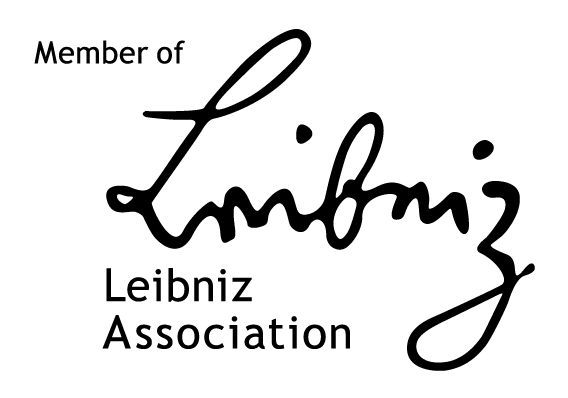
\includegraphics[width=21mm]{figures/logo_leibniz}
      % };
    }
  }
  \ifthenelse{\equal{#1}{1}}{}{
    \vbox to \borderheight {}
  }
}

\DeclareDocumentCommand{\zoomoverlay}{ m }{
  \tikz[baseline,overlay]{
    \path[fill=white] ($(current page.west)+(1mm,30mm)$) rectangle ($(current page.center)+(0,-30mm)$);
    % \tikzset{
    % photo/.style={
    % inner sep=0,
    % rounded corners=0.4mm,
    % },
    %   outline/.style={
    %   draw=white,
    %   line width=\outlinewidth*2,
    %   line cap=round
    % }
    % }
    %   \fill[white] ($(current page.center)+(-40mm,30mm)$) rectangle ($(current page.center)+(30mm,-30mm)$);
    %   \insertzoom{USA}{58 349 296 8}{$(current page.center)+(\zoomoverlayshift-\zoomoverlaywidth/2-\zoomoverlaygap/2,\zoomoverlayheight/2+\zoomoverlaygap/2)$}{#1}
    %   \insertzoom{EUR}{279 349 75 8}{$(current page.center)+(\zoomoverlayshift+\zoomoverlaywidth/2+\zoomoverlaygap/2,\zoomoverlayheight/2+\zoomoverlaygap/2)$}{#1}
    %   \insertzoom{ASI}{279 8 75 349}{$(current page.center)+(\zoomoverlayshift+\zoomoverlaywidth/2+\zoomoverlaygap/2,-\zoomoverlayheight/2-\zoomoverlaygap/2)$}{#1}
    %   \insertzoom{AFR}{58 8 296 349}{$(current page.center)+(\zoomoverlayshift-\zoomoverlaywidth/2-\zoomoverlaygap/2,-\zoomoverlayheight/2-\zoomoverlaygap/2)$}{#1}
    \node[inner xsep=5mm,fill=white,xshift=-2mm] at (current page.center) {
      % \includegraphics[width=100mm,clip,trim={111 5 123 5}]{#1}
      \includegraphics[width=100mm,clip,trim={90 5 100 5}]{#1}
    };
  }
}

\define@cmdkeys{citation}{
  authors,
  year,
  title,
  journal,
  volume,
  underreview,
  break,
  type,
}{}
\presetkeys{citation}{
  authors=,
  year=,
  title=,
  journal=,
  volume=,
  underreview=,
  break=,
  type=,
}{}

\DeclareDocumentCommand{\citationformat}{ m }{%
  \setkeys{citation}{#1}%
  \ifthenelse{\equal{\cmdKV@citation@type}{highlight}}{%
    \def\highlightauthor{\culine[0.67pt][-0.5ex]{tableaugray}}%
  }{%
    \ifthenelse{\equal{\cmdKV@citation@type}{highlightschema}}{%
      \def\highlightauthor{\culine[0.67pt][-0.5ex]{tableaugray}}%
    }{%
      \def\highlightauthor{\relax}%
    }
  }
  \cmdKV@citation@authors%
  \ifthenelse{\equal{\cmdKV@citation@year}{}}{%
    .
  }{
    { }(\cmdKV@citation@year).
  }%
  \cmdKV@citation@break
  \ifthenelse{\equal{\cmdKV@citation@type}{long}}{
    \emph{\cmdKV@citation@title}.
    \cmdKV@citation@break
  }{}
  \textbf{\cmdKV@citation@journal}%
  \ifthenelse{\equal{\cmdKV@citation@underreview}{}}{}{
    \cmdKV@citation@underreview
  }%
  \ifthenelse{\equal{\cmdKV@citation@type}{long}}{%
    \ifthenelse{\equal{\cmdKV@citation@volume}{}}{}{%
      , \cmdKV@citation@volume%
    }%
  }{}%
  .%
}

\def\convertto#1#2{\strip@pt\dimexpr #2*65536/\number\dimexpr 1#1}


\definecolor{formulagrey}{HTML}{666666}

\newcommand{\setlistdefaults}[1]{
  \ifthenelse{\equal{#1}{}}{
    \ifnum\@itemdepth=1\relax
    \setlength\itemsep{0.75em}
    \else
    \ifnum\@itemdepth=2\relax
    \setlength\itemsep{0.4em}
    \else
    \ifnum\@itemdepth=3\relax
    \setlength\itemsep{0.3em}
    \fi\fi\fi
  }{
    \setlength\itemsep{#1}
  }
}
\DeclareDocumentEnvironment{enum}{ O{} }{\begin{enumerate} \setlistdefaults{#1}}{\end{enumerate}}
\DeclareDocumentEnvironment{items}{ O{} }{\begin{itemize} \setlistdefaults{#1}}{\end{itemize}}

\tikzstyle{acclimatearrow} = [
arrows={-Stealth},
line width=1.5pt,
draw=tableaugrey!50!black
]

\DeclareDocumentCommand{\insertbackupslides}{ m m }{
  %\begin{frame}
  %  \centering\fontsize{64pt}{64pt}\selectfont
  %  #1
  %\end{frame}
  \input{#2}
}

\DeclareDocumentCommand{\sourcedstatement}{ m m }{
\item
  \begin{minipage}[t]{0.6\textwidth}
    #1
  \end{minipage}
  \hspace{6mm}
  \begin{minipage}[t]{0.3\textwidth}
    \color{black!33!white}
    \fontsize{8pt}{11pt}\selectfont
    #2
    \mbox{}
  \end{minipage}
}

\makeatother

%%% Local Variables:
%%% mode: latex
%%% TeX-master: "../talk"
%%% TeX-command-default: "Make"
%%% End:


\usepackage{xspace} 
\newcommand{\LArrow}{{\Large $\tc{hervor}{\Rightarrow}$~}}
\newcommand{\LASpace}{\\\hspace*{1.6em}}
\providecommand{\herv}[1]{\tc{hervor}{#1}}
\providecommand{\on}[1]{\operatorname{#1}}
\newcommand{\todo}[1]{{\color{red!80!black} TODO: {\itshape\color{orange!70!black} #1}}}
\DeclareRobustCommand{\acclimate}{\emph{acclimate}\xspace}
\DeclareRobustCommand{\Acclimate}{\emph{Acclimate}\xspace}

\usepackage{xspace}  %leerzeichen bei bedarf, aber nicht vor satzeichen
\providecommand{\tc}[2]{\textcolor{#1}{#2}}
\usepackage[]{units}
\providecommand{\myunit}[1]{$\,$\unit{#1}}
\providecommand{\myunitfrac}[2]{$\,\frac{\unit{#1}}{\unit{#2}}$}

%Mathoperators
\newcommand{\E}{\mathbb{E}}
\renewcommand{\P}{\mathcal{P}}
\newcommand{\Var}{\operatorname{Var}}
\newcommand{\DDt}{\operatorname{D_{\Delta t}}}
\newcommand{\tDDt}{\operatorname{\tilde{D}_{\Delta t}}}

\newcommand{\Cov}{\operatorname{Var}}
\newcommand{\mbR}{\mathbb{R}}
\newcommand{\mcF}{\mathcal{F}}
%\newcommand{\argmin}{\operatornamewithlimits{argmin}}
\newcommand{\argmax}{\operatornamewithlimits{argmax}}
\renewcommand{\minof}[2]{\min\left[#1\,,\,#2\right]}
\newcommand{\minofthree}[3]{\min\left[#1\,,\,#2\,,\,#3\right]}
\renewcommand{\maxof}[2]{\max\left[#1\,,\,#2\right]}

\newcommand{\first}{1^{\operatorname{st}}}
\newcommand{\secnd}{2^{\operatorname{nd}}}
\newcommand{\third}{3^{\operatorname{rd}}}
\newcommand{\nth}{\text{n}^{\operatorname{th}}}
%\newcommand{\hPSD}{\hyperlink{PSD}{PSD}\xspace}

%##########################
% Real and imaginary parts
%##########################
\renewcommand{\Re}{\operatorname{Re}}
\renewcommand{\Im}{\operatorname{Im}}
%#############################
% Quantities
%#############################
\newcommand{\DA}{D^A}
\newcommand{\DK}{D^K}
\newcommand{\bA}{\beta^A}
\newcommand{\dA}{\delta^A}

\newcommand{\newleftside}{\ifthenelse{\isodd{\thepage}}{\newpage}{\newpage\phantom{placeholder}\thispagestyle{empty} \newpage}}
\newcommand{\newrightside}{\ifthenelse{\isodd{\thepage}}{\newpage\phantom{placeholder}\thispagestyle{empty} \newpage}{\newpage}}
%
\DeclareCaptionLabelFormat{cont}{#1~#2~(cont.)}

\newcommand{\define}{:=}
\newcommand{\set}{:=}
\newcommand{\from}{\leftarrow}
\renewcommand{\to}{\rightarrow}
\newcommand{\bndollar}[1]{\$#1bn}

\makeatletter
\newcommand{\colorwave}[1][blue]{\bgroup \markoverwith{\lower3.5\p@\hbox{\sixly \textcolor{#1}{\char58}}}\ULon}
\font\sixly=lasy6
\makeatother
\newcommand{\todoline}{\colorwave[red]}

\newcommand{\captioncr}{{\protect\\}}
\AtBeginDocument{\renewcommand\appendixname{Appendix~}}
\def\UrlBreaks{\do\/\do-\/\do_}

\makeatletter
% for aligning in math modes:
\newcommand{\pushright}[1]{\ifmeasuring@#1\else\omit\hfill$\displaystyle#1$\fi\ignorespaces}
\newcommand{\pushcenter}[1]{\ifmeasuring@#1\else\omit\hfill$\displaystyle#1$\hfill\fi\ignorespaces}
\newcommand{\pushleft}[1]{\ifmeasuring@#1\else\omit$\displaystyle#1$\hfill\fi\ignorespaces}
% instead of eqnarray use:
% \begin{alignat}{4} a&&\pushcenter{=}&b \end{alignat}
\makeatother

\newcommand{\annot}[2][]{%
  \pdfannot width \linewidth height 2\baselineskip depth 0pt{%
    /Subtype/Text%
    /Open false
    /Name /Comment%
    /CA .4%
    /C [.3 .6 .9]%
    /T (\pdfescapestring{#1})%
    /Contents(\pdfescapestring{\detokenize{#2}})%
  }
}
\ifdefined\note\relax\else
\newcommand\note[1]{\marginnote{\begin{minipage}{0.8\marginparwidth}\footnotesize\raggedright{}#1\end{minipage}}}
\fi

%#############################
% Sets
%#############################
\newcommand{\mbC}{\mathbb{C}}
\newcommand{\mbN}{\mathbb{N}}
\newcommand{\mbDA}{\mathbb{D}^A}
%%%%%%%%%%%%%%%%
% Farben
%%%%%%%%%%%%%%%%
\definecolor{dunkelgrau}{rgb}{0.8,0.8,0.8}
\definecolor{hellgrau}{RGB}{204,216,226}

\newcommand{\citationfloodingadaptation}{
  \textcolor{black!60!white}{Willner, Levermann, Zhao, Frieler.}
  \emph{Science Advances}.
  \textcolor{black!60!white}{2018 (OA)}
}

%%%%%%%%%%%%%%%%%%%%%%%%%%%%%%%%%%%%%%%%%%%%%%%%%%%%%%%%%%%%%%%%%%%%%%%%%%%%%% 

\author{Christian Otto, T. Geiger, and Katja Frieler}
\title{Climate Impacts in Macroeconomic Growth Models}
\date{$\secnd$ Damage Meeting, June 11}
\hypersetup{pdfauthor={Christian Otto}}

\begin{document}

\begin{frame}[plain]
  \maketitle
\end{frame}
%%%%%%%%%%%%%%%%%%%%%%%%%%%%%%%%%%%%%%%%%%%%%%%%%%%%%%%%%%%%%%%%%%%%%%%%%%%%%% 
\begin{frame}
  \frametitle{Possible Ways Forward}
  \begin{enumerate}
  \item Empirically estimate relative importance and persistencies of impact channels (e.g., capital stock, total factor productivities, labor productivity etc.) accounted for in IAMs at different levels of global warming
  \item Estimate cumulative GDP losses for each levels of warming and use these as IAM input
  \item Endogenously explain empirically observed persistencies by `specialized' impact models 
  \end{enumerate}
  \begin{itemize}
\arrowitem 1. appears to be feasible way forward for next evaluation
  \end{itemize}
\end{frame}

\begin{frame}
  \frametitle{Production Functions in IAMs}
  \begin{itemize}
  \item  Production system in IAMs often described by an aggregate production function of CES or Cobb-Douglas type
  \end{itemize}
  \vfill
  \begin{equation*}
    \label{eq:CD}
    Y(\tau,T)\equiv \big(1-\tc{red}{\DA(\tau,T)}\big)A(\tau)\left[\big(1-\tc{red}{\DK(\tau,T)}\big)K(\tau) \right]^\alpha L(\tau)^{\alpha-1}
  \end{equation*}
  \vfill
  \begin{minipage}[l]{.45\linewidth}
 % \begin{adjustwidth}{-\leftframemargin}{-\rightframemargin}
   \begin{itemize} 
   \item [$\tau$] Slow (decadal) timescale
   \item [$T$] Global temperature
 %  \item [$A$] Total factor productivity
 %  \item [$K$] Capital
  % \item [$L$]  Labor
  % \item [$\alpha$] Cobb-Douglas coefficient
   \end{itemize}
 %\end{adjustwidth}
\end{minipage}\hfill
\begin{minipage}[l]{.45\linewidth}
  \begin{itemize}
  \item [$\tc{red}{\DA}$] \tc{red}{Relative} damages to $A$ 
   \item [$\tc{red}{\DK}$] \tc{red}{Relative} damages to capital
   \end{itemize}
 \end{minipage}
 
 \vfill
 \begin{itemize}
 \item Assumption: Climate extremes have an instantaneous impact on $K$, and have persistent impacts on $A$, GDP.
   \arrowitem Estimate persistencies for $A$
   \end{itemize}
\end{frame}


\begin{frame}
  \frametitle{Climate Damages From ISIMIP Simulations}
  \begin{enumerate}
  \item Estimate persistence times
  \item Sum damages across categories
  \item Obtain timeseries of cumulative damages (country or subnational level)
  \item Transition From event-based to temperature dependent damages
  \item Integrate to world regions  
  \end{enumerate}
\end{frame}

\begin{frame}
  \frametitle{Step 1: Estimate Persistencies}
  \begin{minipage}[r]{.6\linewidth}
    \vspace{0pt}
  \begin{itemize}
  \item Panel regressions with time lags
  \end{itemize}
  \begin{equation*}
    \ln\big(A_{j,t} \big) = \gamma_j + \delta_{t} + \theta_j t + \sum_{l=0}^{L}\tc{red}{\bA_{l}E_{j,t-l}}+\epsilon_{j,t}
  \end{equation*}
  \begin{adjustwidth}{+.5\leftframemargin}{+.5\rightframemargin}
    \begin{itemize}
  \item[$\tc{red}{E_{j,t}}$] Biophysical hazard indicator\\ (e.g., windspeed for trop. cyclones)
  \end{itemize}
\end{adjustwidth}
\begin{itemize}
  \item Cumulative impact $k$ years after exposure
  \end{itemize}
  \begin{equation*}
    \Omega_{t,k}\equiv\sum_{l=0}^{k}\beta_{t-L}
  \end{equation*}
  \begin{sources}
    \item Hsiang, 2014
  \end{sources}
\end{minipage}\hfill
\begin{minipage}[r]{.39\linewidth}
    \vspace{-30pt}
  \centering
  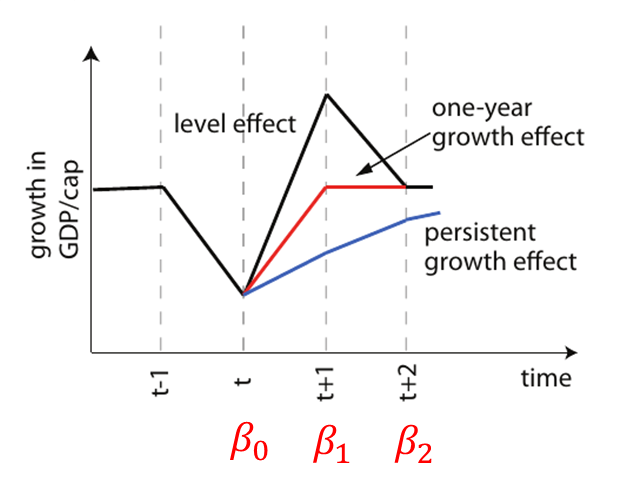
\includegraphics[width=.75\textwidth]{figures/sketch_let_effect}
  \vfill
  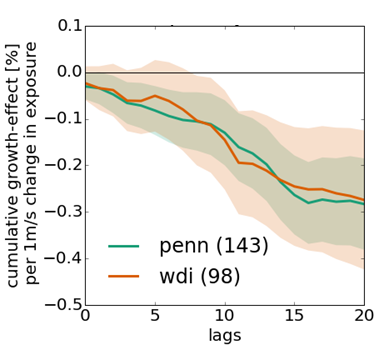
\includegraphics[width=.75\textwidth]{figures/ind_windspeed}
\end{minipage}
\end{frame}

\begin{frame}
  \frametitle{Step 2: Sum Damages Across Categories}
  \begin{minipage}[t]{.6\linewidth}
    \vspace{0pt}
  \begin{itemize}
  \item Affected people \tc{red}{$P_j$} as unified hazard indicator across categories
  \end{itemize}
  \begin{equation*}
    \ln\big(A_{j,t}\big) = \gamma_j + \delta_{t} + \theta_j t + \sum_{l=0}^{L}\bA_{l}\tc{red}{P_{j,t-l}}+\epsilon_{j,t}
  \end{equation*}
  \begin{itemize}
  \item Cumulative impact $k$ years after exposure
  \end{itemize}
  \begin{equation*}
    P_{i,t-l}\equiv\frac{1}{\operatorname{Pop}_{i,t-l}}\sum_{c\in\mbC} P_{i,t-L}
  \end{equation*}
\end{minipage}\hfill
\begin{minipage}[t]{.39\linewidth}  
  \vspace{-30pt}
  \raggedleft
  \tc{tableaublue}{Indicator: windspeed}
  \centering
  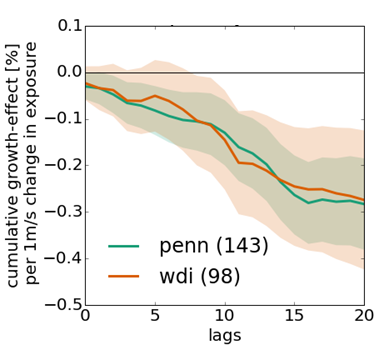
\includegraphics[width=.6\textwidth]{figures/ind_windspeed}
  \vfill
  \raggedleft
  \tc{tableaublue}{Indicator: Affected people}
  \centering
  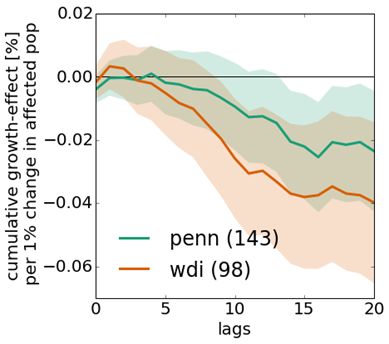
\includegraphics[width=.6\textwidth]{figures/ind_affected_people}
\end{minipage}
\end{frame}

\begin{frame}
  \frametitle{Step 3: Timeseries of Cumulative Damages}
      \begin{minipage}[l]{\linewidth}
        \begin{itemize}
  \item For simplicity assume:\\ 1 GCM $+$ SSP2 $+$ 1 impact model for each category $c\in\mbC$          
  \item Timeseries of \emph{relative} cumulative damages for country $j$ for \emph{one} impact realization up to time $t$ $\lbrace P\rbrace_{j,t}$  
  \end{itemize}
  \begin{equation*}
     \DA_{j,t}\left(\lbrace P\rbrace_{j,t}\right)\equiv 1 - \ \prod_{n=0}^{t}\left(1-\dA_{j,t-n}\right)
   \end{equation*}
   \begin{itemize}
\item  $\dA_{j,t-n}$ denotes the `instantaneous' damage caused by a series $\lbrace P_{j,t-m}^i\rbrace_{m=0}^L$ of hazards   
   \end{itemize}
  \begin{equation*}
    \dA_{j,t}\left(\lbrace P_{j,t-m}^i\rbrace_{m=0}^L\right)\equiv \sum_{m=0}^L\beta_m\sum_{i=0}^IP_{j,t-m}^i
  \end{equation*}
%   \begin{itemize}
% \arrowitem Average over the different impact model combinations?
%   \end{itemize}

\end{minipage}\hfill
\begin{minipage}[r]{0\linewidth}
\end{minipage}
\end{frame}

\begin{frame}
  \frametitle{Step 4: From Event-Based to Temperature Dependent Damages}
  \begin{minipage}[t]{.65\linewidth}
    \vspace{0pt}
  \begin{itemize}
  \item Each RCP-SSP-GCM combination provides \textbf{unique} mapping $t \mapsto T$
    \arrowitem For each temperature interval $\Delta T$ there is associated set of cumulative damages
  \end{itemize}
    \begin{equation*}
   \mbDA_{j}(\Delta T)\equiv\lbrace \DA_{j,t}\, \vert\, t' \text{ for } T(t')\in\Delta T \rbrace
 \end{equation*}
 \vspace{-20pt}
\begin{itemize}
\item Ensemble average over set members $\mbDA_{j}(\Delta T)$ yields country level damages over temperature interval  
\end{itemize}
\begin{equation*}
  \langle \DA_{j}\rangle(\Delta T)\equiv\big\langle \DA_{j,t}\big\rangle_{\mbDA_{j}}(\Delta T)
\end{equation*}
\end{minipage}\hfill
\begin{minipage}[t]{.35\linewidth}
  \vspace{20pt}
  \centering
  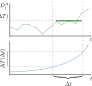
\includegraphics[width=\linewidth]{figures/damage_averaging}
\end{minipage}
\end{frame}

\begin{frame}
  \frametitle{Step 5: Integration to World Regions}
  \begin{itemize}
  \item IAMs operate on the level of world regions $r\in\mbN_r$
    \arrowitem Average over the countries $j$ belonging to each region $r$ (weighted by average population or GDP or asset stock to obtain damages $\langle \DA_{r}\rangle(\Delta T)$ for $\Delta T$.
  \end{itemize}

  \begin{itemize}
  \item For each RCP-SSP combination average IAM output over different GCM-Impact model combinations
  \end{itemize}
  
\end{frame}
%%%%%%%%%%%%%%%%%%%%%%%%%%%%%%%%%%%%%%%%%%%%%%%%%%%%%%%%%%%%%%%%%%%%%%%%%%%%%%

\end{document}



% \begin{frame}[label=adaptationbins]
%   \frametitle{Necessary adaptation to keep historic risk in 2035--2044}
%   \vspace{-2.5mm}
%   \begin{adjustwidth}{-\leftframemargin}{-\rightframemargin}
%     \centering
%     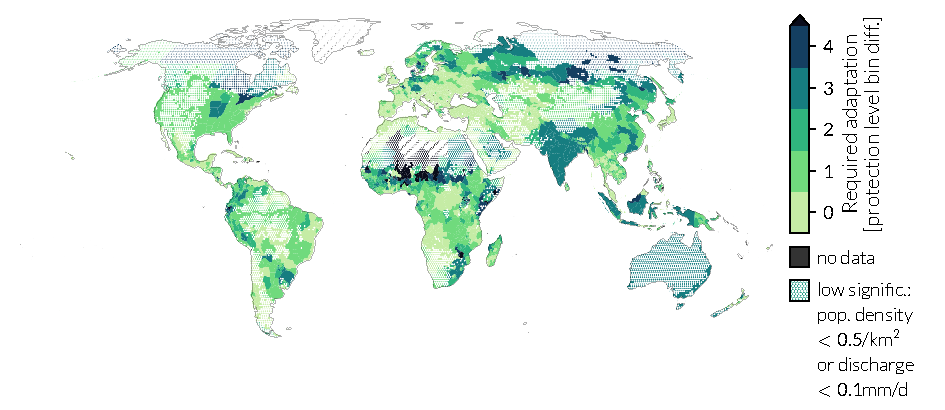
\includegraphics[width=14.5cm]{figures/adaptation/map_protection_bins_shift_masked.pdf}
%     %\drawmapcorrection
%   \end{adjustwidth}
%   \vspace{-4mm}
%   \begin{messages}[-8mm]
%     \arrowitem Highest adaptive pressure in India and Indonesia
%     \arrowitem Also some rich countries have to adapt
%   \end{messages}
%   \begin{sources}
%   \item[] \citationfloodingadaptation
%   \end{sources}
% \end{frame}


%%% Local Variables:
%%% mode: latex
%%% TeX-master: t
%%% TeX-command-default: "Make"
%%% End:
